\documentclass[11pt]{article}

\newcommand{\cnum}{CM146}
\newcommand{\ced}{Fall 2017}
\newcommand{\ctitle}[3]{\title{\vspace{-0.5in}\cnum, \ced\\Problem Set #1: #2\\Due #3}}
\usepackage{enumitem}
\newcommand{\solution}[1]{{{\color{blue}{\bf Solution:} {#1}}}}
\usepackage[usenames,dvipsnames,svgnames,table,hyperref]{xcolor}
\usepackage{graphicx, amsmath}
\renewcommand*{\theenumi}{\alph{enumi}}
\renewcommand*\labelenumi{(\theenumi)}
\renewcommand*{\theenumii}{\roman{enumii}}
\renewcommand*\labelenumii{\theenumii.}

\graphicspath{ {images/}}

\begin{document}
\ctitle{2}{Atibhav Mittal (804598987)}{Feb 6,2017}
\author{}
\date{}
\maketitle
\vspace{-0.75in}

\section{Problem 1}
\begin{enumerate}
\item 

\solution{} \newline
Consider a function $f = x_1 + x_2 - 1.5$ \newline
This is a valid perceptron for the AND function. \newline
Another valid perceptron could be $g = x_1 + x_2 - 1.9$ \newline
Both of these predict negative values for when the output of the AND function is 0, 
and positive values when the output of AND is 1.

\item 
\solution{} \newline
There does not exist any valid perceptron that works for the XOR function. \newline
This is because the data is not linearly separable, positive and negative examples
are opposite corners of the unit square.

\end{enumerate}

\newpage
\section{Problem 2}
\solution{} 
$$
\frac{\partial J(\theta)}{\partial \theta_j} = \frac{\partial}{\partial \theta_j} \left(- \sum_{n=1}^N y_n \log h_{\theta} (x_n) + (1 - y_n) \log (1 - h_{\theta} (x_n)) \right)
$$
$$
\frac{\partial J(\theta)}{\partial \theta_j} = - \sum_{n=1}^N \frac{\partial}{\partial \theta_j} \left( 
	y_n \log h_{\theta} (x_n) + (1 - y_n) \log (1 - h_{\theta} (x_n))
\right)
$$
We can first compute the derivative of $h_{\theta}(x_n)$
$$
	\frac{\partial h_{\theta}(x_n)}{\partial \theta_j} = \frac{\partial}{\partial \theta_j} (\sigma (w^T x_n)) = \sigma(w^T x_n) (1 - \sigma (w^T x_n)) x_{n,j}
$$
$$
\Rightarrow	\frac{\partial h_{\theta}(x_n)}{\partial \theta_j} = h_{\theta} (x_n) (1 - h_{\theta} (x_n)) x_{n,j}
$$
$$
\frac{\partial J(\theta)}{\partial \theta_j} = - \sum_{n=1}^N  \left[ 
	\frac{\partial}{\partial \theta_j} (y_n \log h_{\theta} (x_n) ) + \frac{\partial}{\partial \theta_j} ( 1 - y_n) \log (1 - h_{\theta} (x_n))
\right]
$$
$$
\frac{\partial J(\theta)}{\partial \theta_j} = - \sum_{n=1}^N  \left[ 
	\frac{y_n}{h_{\theta}(x_n)} \cdot h_{\theta} (x_n) (1 - h_{\theta} (x_n)) x_{n,j} + 
	\frac{1 - y_n}{1 - h_{\theta}(x_n)} \cdot (- h_{\theta} (x_n) (1 - h_{\theta} (x_n)) x_{n,j} )
\right]
$$
$$
\frac{\partial J(\theta)}{\partial \theta_j} = - \sum_{n=1}^N  x_{n,j} \left[ 
	y_n (1 - h_{\theta} (x_n)) - (1 - y_n) h_{\theta} (x_n) 
\right]
$$
$$
\frac{\partial J(\theta)}{\partial \theta_j} = - \sum_{n=1}^N  x_{n,j} \left[ 
	y_n - h_{\theta}(x_n)
\right]
$$
\newpage
\section{Problem 3}
\begin{enumerate}
\item
\solution{} 
$$
\frac{\partial J}{\partial \theta_0} = \sum_{n=1}^N w_n 2 (\theta_0 + \theta_1 x_{n,1} - y_n) = 2 \sum_{n=1}^N w_n (\theta_0 + \theta_1 x_{n,1} - y_n)
$$
$$
\frac{\partial J}{\partial \theta_1} = \sum_{n=1}^N w_n 2 (\theta_0 + \theta_1 x_{n,1} - y_n) \cdot x_{n,1} = 
2 \sum_{n=1}^N w_n (\theta_0 + \theta_1 x_{n,1} - y_n) \cdot x_{n,1}
$$

\item
\solution{} \newline
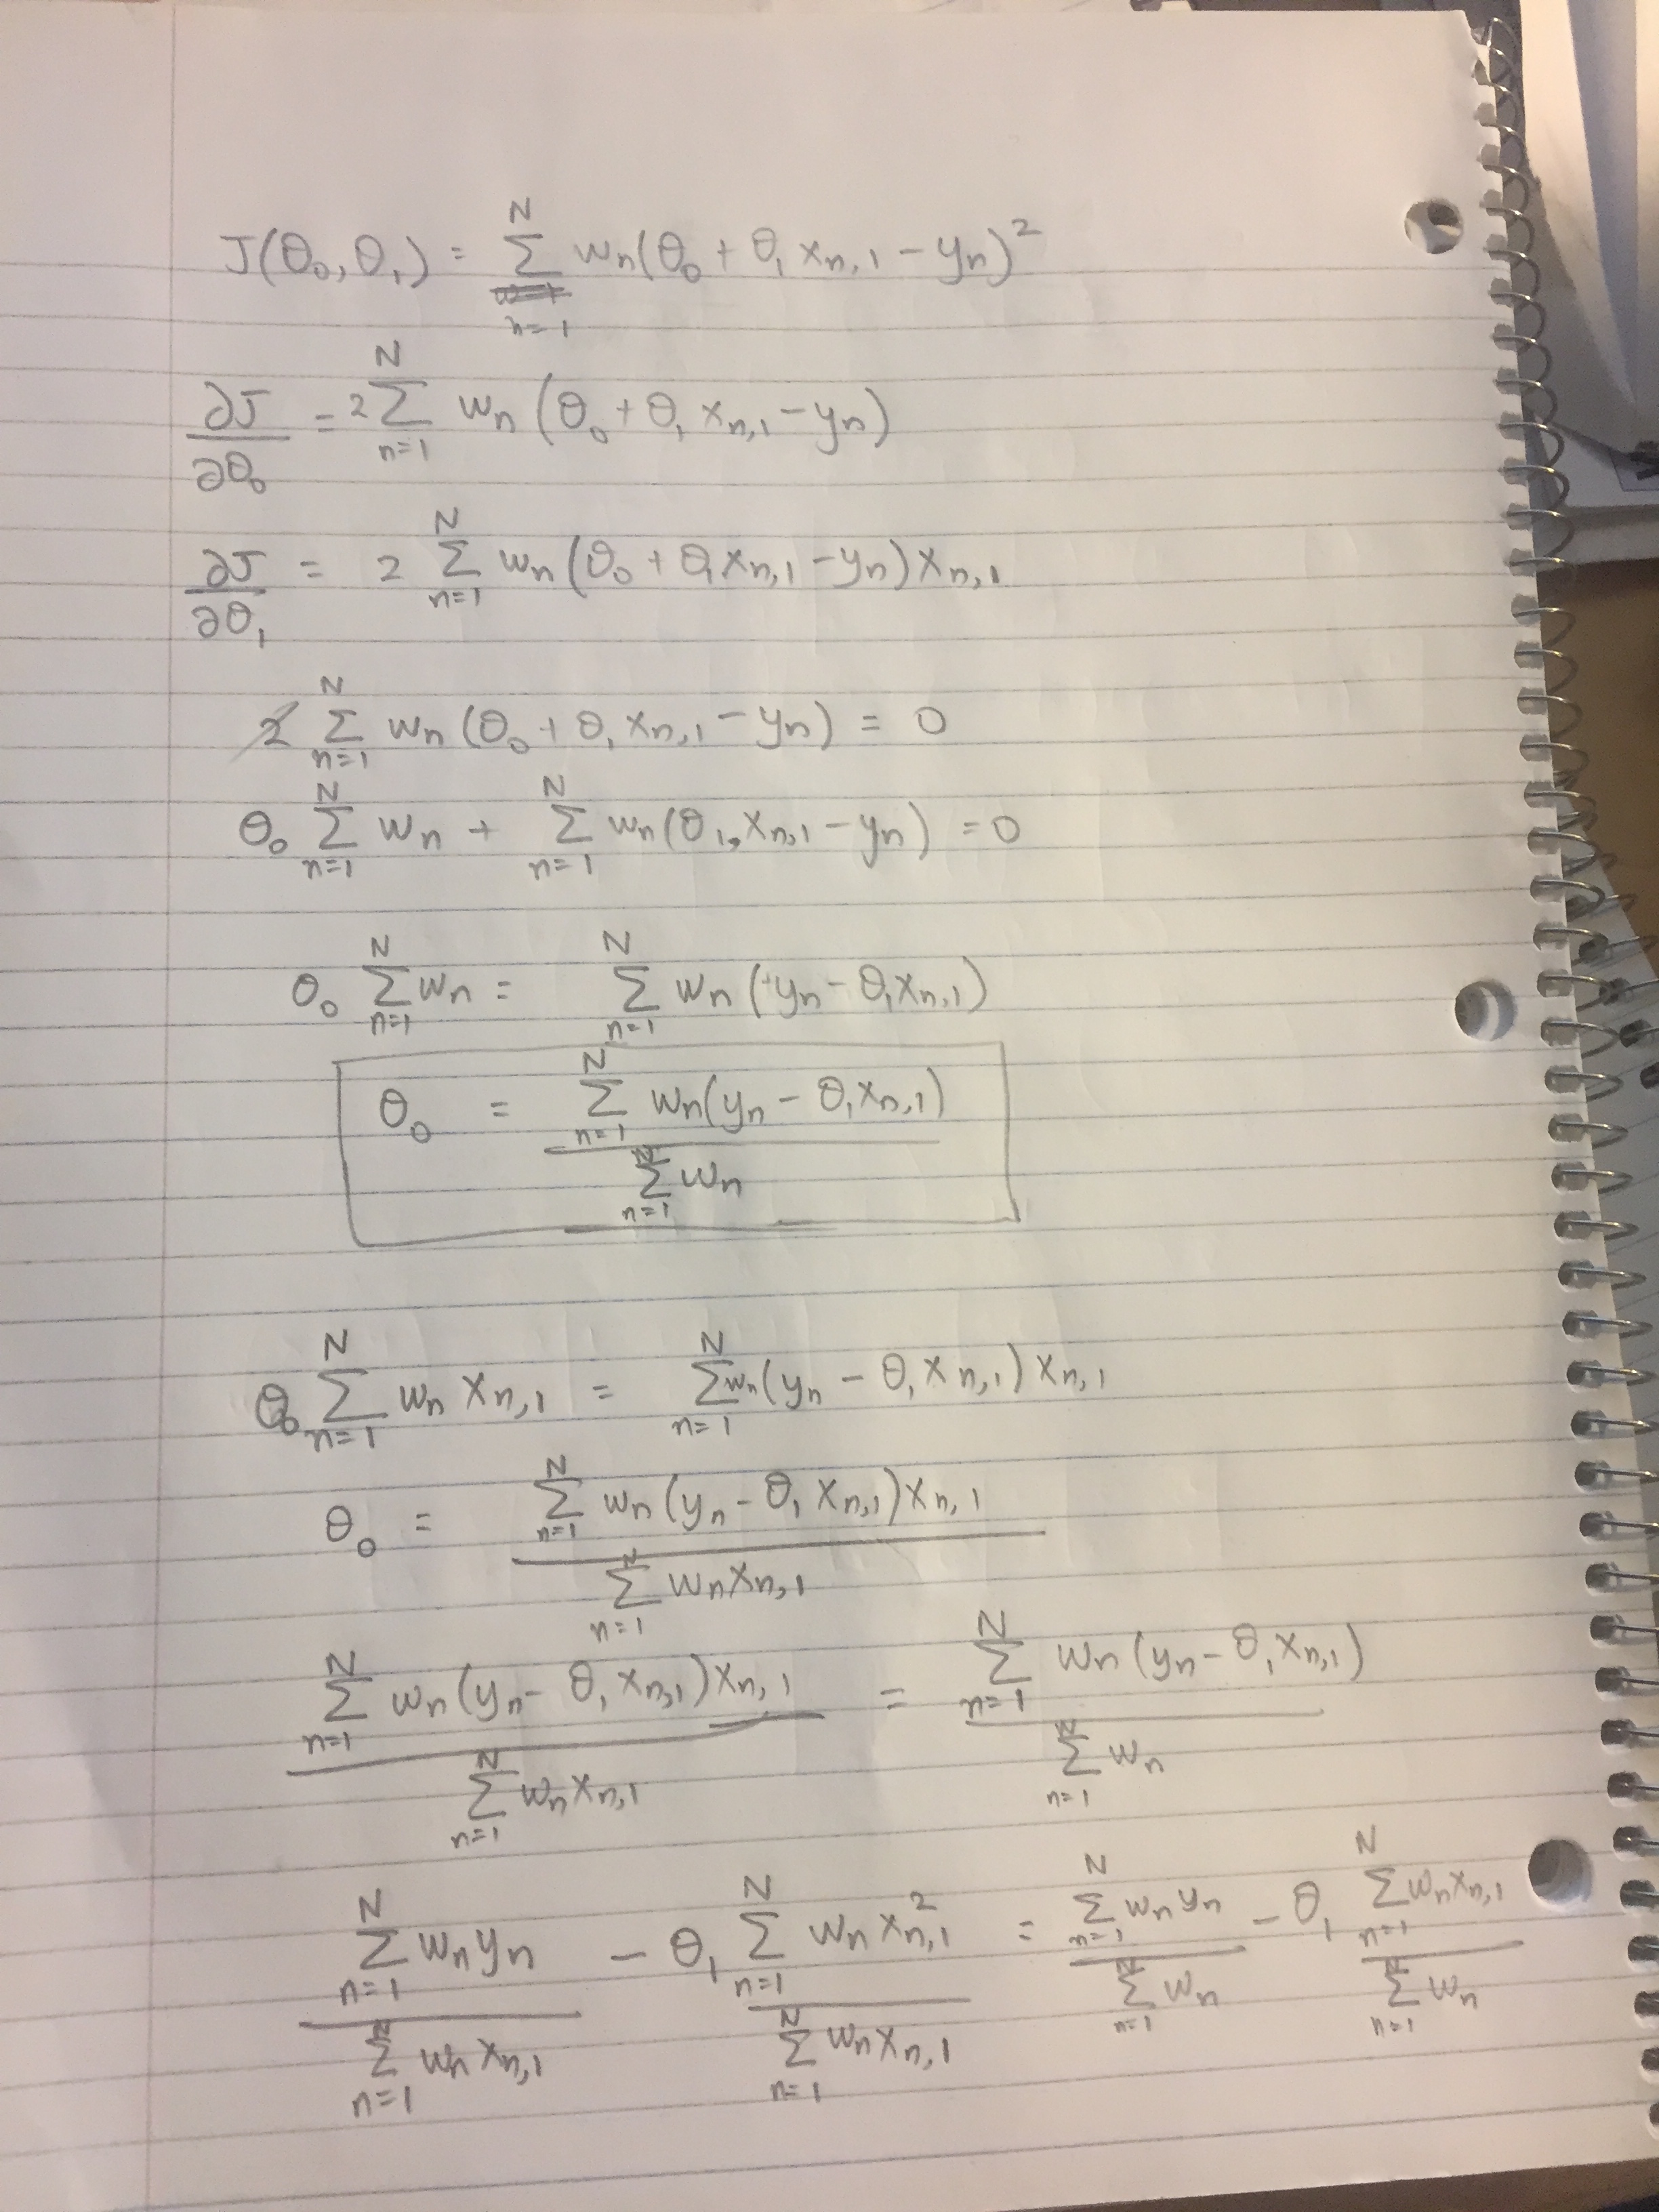
\includegraphics[scale=0.1]{3b_1.jpg} \newline
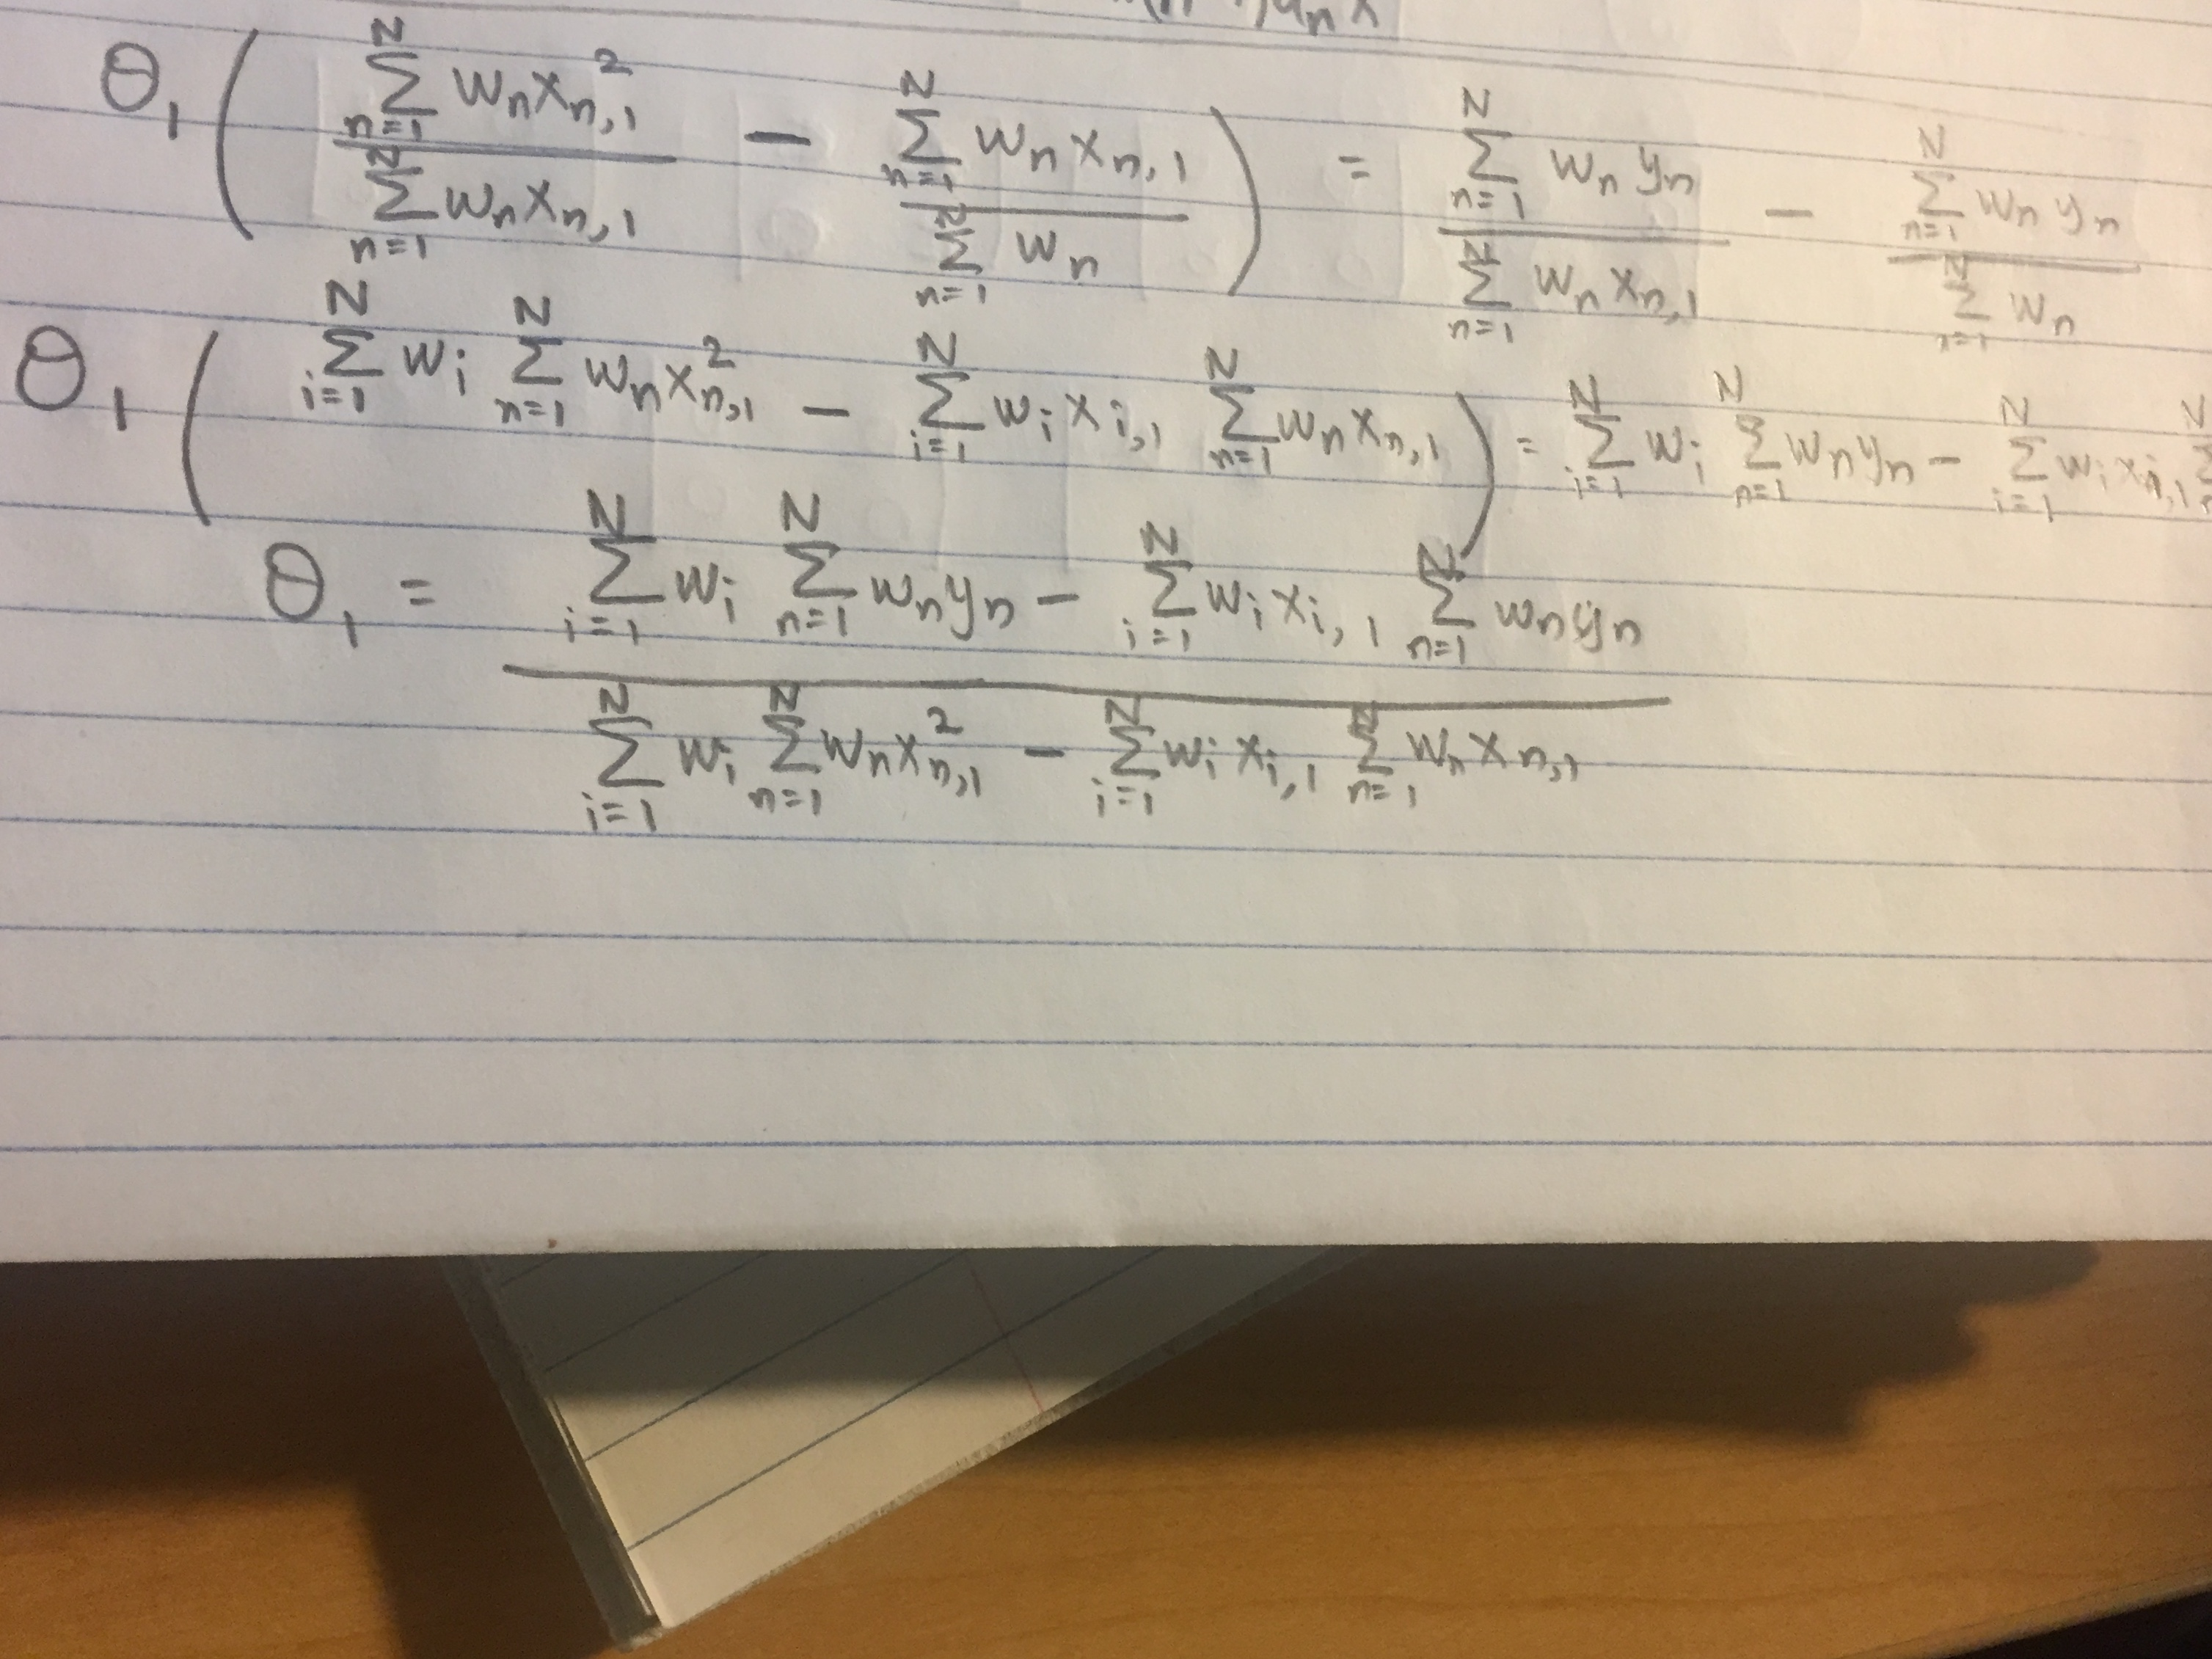
\includegraphics[scale=0.1]{3b_2.jpg} \newline
Using the above work, we get the following expression for $\theta_1$
$$
\theta_1 = 
\frac{
\sum_{i=1}^N w_i \sum_{n=1}^N w_n y_n - \sum_{i=1}^N w_i x_{i,1} \sum_{n=1}^N w_n y_n
}{
\sum_{i=1}^N w_i \sum_{n=1}^N w_n x_{n,1}^2 - \sum_{i=1}^N w_i x_{i,1} \sum_{n=1}^N w_n x_{n,1}
}
$$

We can plug this value into the value for $\theta_1$ in the equation below to solve for $\theta_0$
$$
\theta_0 = 
\frac{\sum_{n=1}^N w_n y_n}{\sum_{n=1}^N w_n} - \theta_1 \frac{\sum_{n=1}^N w_n x_{n,1}}{\sum_{n=1}^N w_n}
$$
$$
\theta_0 = 
\frac{\sum_{n=1}^N w_n y_n}{\sum_{n=1}^N w_n} - 
\left(
\frac{
\sum_{i=1}^N w_i \sum_{n=1}^N w_n y_n - \sum_{i=1}^N w_i x_{i,1} \sum_{n=1}^N w_n y_n
}{
\sum_{i=1}^N w_i \sum_{n=1}^N w_n x_{n,1}^2 - \sum_{i=1}^N w_i x_{i,1} \sum_{n=1}^N w_n x_{n,1}
} \right)
 \frac{\sum_{n=1}^N w_n x_{n,1}}{\sum_{n=1}^N w_n}
$$
The above values minimize the value of $J(\theta_0, \theta_1)$
\end{enumerate}
\newpage

\section{Problem 4}
\begin{enumerate}
\item 
\solution{} \newline
Since D is linearly separable, consider $\bar{w}, \bar{\theta}$ that satisfy (1).
Consider $w = a \bar{w} , \theta = a \bar{\theta} + b$. To satisfy
the condition of the LP, \newline
if $y_i = 1$: 
$$
	a(\bar{w}^T x_i + \bar{\theta}) + b \geq 1 - \delta 
$$ \newline
$ 
\Rightarrow
	aC + b \geq 1 - \delta 
$ for some C $\geq$ 0 \newline
Since $ \delta > 0$, the inequality becomes:
$$
	aC + b \geq 1
$$
if $y_i = - 1$:
repeating the above steps, we get the inequality: \newline
$
aM - b \geq 1
$ for some positive constant M \newline
Both of these inequalities will be satisified if the second inequality is satisfied. (if $a, b > 0$)
Hence, there exists infinitely many solutions to this inequality.
Since its a greater than inequality, and we are trying to minimize $\delta$, the value of $\delta = 0$
produces a solution to this.
Since $\delta \geq 0$, this is the optimal solution

\item 
\solution{} \newline
Since there exists an optimal solution $\delta = 0$, we have:
$$
y_i (w^T x_i + \theta ) \geq 1 - \delta = 1
$$
if $y_i$ = 1: 
$$
 w^T x_i + \theta \geq 1 \geq 0
$$
if $y_i = -1$:
$$
	(-1)(w^T x_i + \theta) \geq 1
$$
$$
	w^T x_i + \theta < -1 < 0
$$
Hence, both the conditions for (1) are satisfied. Thus the data is linearly separable

\item 
\solution{} \newline
If there exists a hyperplane that satisfies (2) with $\delta > 0$, then we know that 
the data is not as further apart as would be optimal. Hence, it means that there is
still a hyperplane that separates the data but the two classes of data are closer to 
each other (i.e. smaller margin).

\item
\solution{} \newline
The optimal solution to this LP formulation is always $\delta = 0$. Hence, it gives us
no method to find a good linear separator, which is what we want to do with the LP 
formulation. If we use the given LP formulation, then the LP formulation is reduced to
the same condition we had in (1).

\item
\solution{} \newline
The optimal hyperplane for this D would be one that passes through opposite ends
of the unit cube. This corresponds to
$$
w = 
\begin{bmatrix}
1 \\
1 \\
1
\end{bmatrix}
 \theta =
\begin{bmatrix}
0 \\
0 \\
0
\end{bmatrix}
, \delta = 1
$$

\end{enumerate}

\newpage

\section{Problem 5}
\begin{enumerate}
\item
\solution{} \newline
Training Data Graph \newline
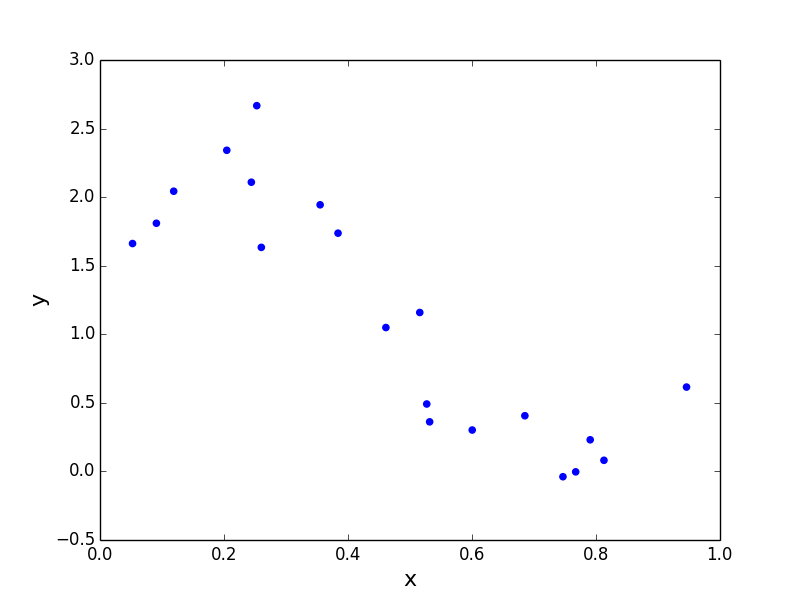
\includegraphics[scale=0.4]{train.png} \newline
Test Data Graph \newline
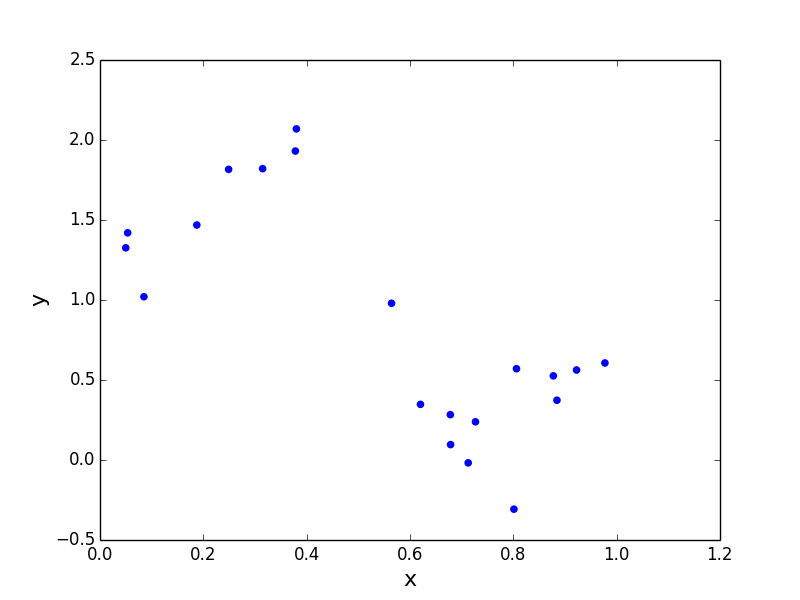
\includegraphics[scale=0.4]{test.png} \newline
From the above visualization, there seems to be a line with a negative slope that would fit the 
test data quite well. The same line would pass through the center of a lot of points in the test
data. However, there seems to be more scattering of points in the test data as compared to the 
train data, which might lead to a poorer fit as compared to the training data. \newline
Overall, I think linear regression might be effective in predicting the data.

\item - (d)
\solution{} \newline
\begin{tabular}{| c | c | c | c |}
\hline
Step Size $\eta$ & Coefficients & Num. Iterations & Final Value \\
\hline 
0.01 & 2.44640703 -2.81635347 & 766 & 3.91257640579 \\
\hline
0.001 & 2.44640684 -2.81635307 & 7077 & 3.91257640579 \\
\hline
0.0001 & 2.27044798 -2.46064834 & 10000  & 4.0863970368 \\
\hline
0.0407 &  -9.40470931e+18  -4.65229095e+18 & 10000 & 2.71091652001e+39 \\
\hline
\end{tabular}
The above results show that eta, with a step size of 0.01 converges the quickest, 
and a step size of 0.001 converges, but slower than that of 0.01. When we set our
step size to 0.0001, we can notice that the coefficients and the objective function
value are approaching the convergence value, but does not reach it within 10000 
iterations. \newline
For a step size of 0.0407, we notice an extremely large value for the objective 
function and also for the coefficients. This is due to gradient descent overshooting
the optimal value, which leads to increasing coefficients. Hence, it does not converge
for a step size of 0.0407.
\addtocounter{enumi}{2}

\item
\solution{} \newline
The solution we get from the closed form optimization is: \newline
Coefficients = 2.44640709 -2.81635359
Final Value of Loss function = 3.91257640579
Comparing these to the values obtained from Gradient Descent, we observe
that the final value of the loss function is identical. The coefficients
differ by an extremely minimal amount ($2.54 * 10^{-6} \%$). This is likely
due to a rounding error. \newline
I timed both the fitting processes using Python's time module, to see how
long it takes for either process to converge. 
Gradient Descent (Step size = 0.01): 0.035s
Closed Form: 0.0013s
The closed form solution is much faster, since there is no looping involved.

\item
\solution{} \newline
Using a variable step size gives us the following result: \newline
Coefficients: 2.44640679 -2.81635297 \newline
Final Cost: 3.91257640579 \newline
Number of Iterations: 1409 \newline
This approach yields almost the same results as the closed form optimization
(differences could be attributed to rounding error). However, it takes more
iterations than a constant step-size gradient descent.

\item - (h)
\solution{} \newline
Using RMSE might be better than using $J(\theta)$ because 
\begin{enumerate}
	\item It divides by the number of examples, giving us the error per example
		  which is a better measure of error than just the total sum
	\item It increases the cost by a large amount if the prediction is way different
		  than the actual value. This might not be seen if we use just $J(\theta)$.
\end{enumerate}

\addtocounter{enumi}{1}

\item 
\solution{} \newline
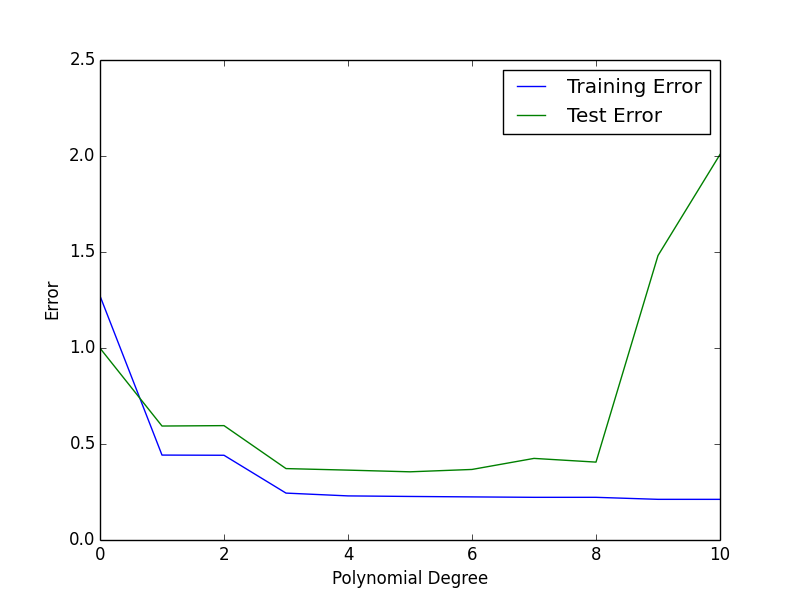
\includegraphics[scale=0.6]{5i.png} \newline
From the above plot, a polynomial of degree between 4 and 6 would be a good choice.
This is because it has both low training and low test error. \newline
There is evidence of both underfitting and overfitting. \newline
The underfitting can be observed in the left part of the graph where the training error 
is huge. This is due to the fact that the polynomial is not complex enough to find a 
good decision boundary. \newline
Overfitting can be observed in the right part of the graph, after polynomial of degree 8.
This is due to the fact that the model finds intricacies to try and best fit the training
data. However, due to this, the model doesn't generalize well and results in large test
error, and thus overfitting.
\end{enumerate}


\end{document}
